
\newpage
{\large 2022 - 0} (Řešeno společně na tabuli na poslední přednášce.)

\begin{questions}

\question Napište definici grupy.
\question Mějme zobrazení \(f: A \rightarrow B\) a zobrazení \(g: B \rightarrow C\). Dále máme zobrazení \(h = g \circ f\) (\(g\) po \(f\)). Je-li \(h\) injekce, plyne z toho, že \(f\) a \(g\) jsou injekce?
\question Napište příklad vektorového prostoru, kde jsou jen 2 vektory.
\question Jakých hodnot může nabývat stopa reálné antisymetrické matice?
\question Napište definici vnitřního součinu na reálném vektorovém prostoru.
\question Uveďte zcela přesně podmínku, kdy je soustava lineárních rovnic řešitelná.

\end{questions}

\hrule

\begin{questions}

{\color{gray}

\question Grupa je množina s jednou operací, pro kterou platí
\begin{enumerate}
    \item asociativita
    \item existence neutrálního prvku
    \item pro všechny členy množiny existuje inverzní prvek
\end{enumerate}

\question Neplyne.

\begin{center}
    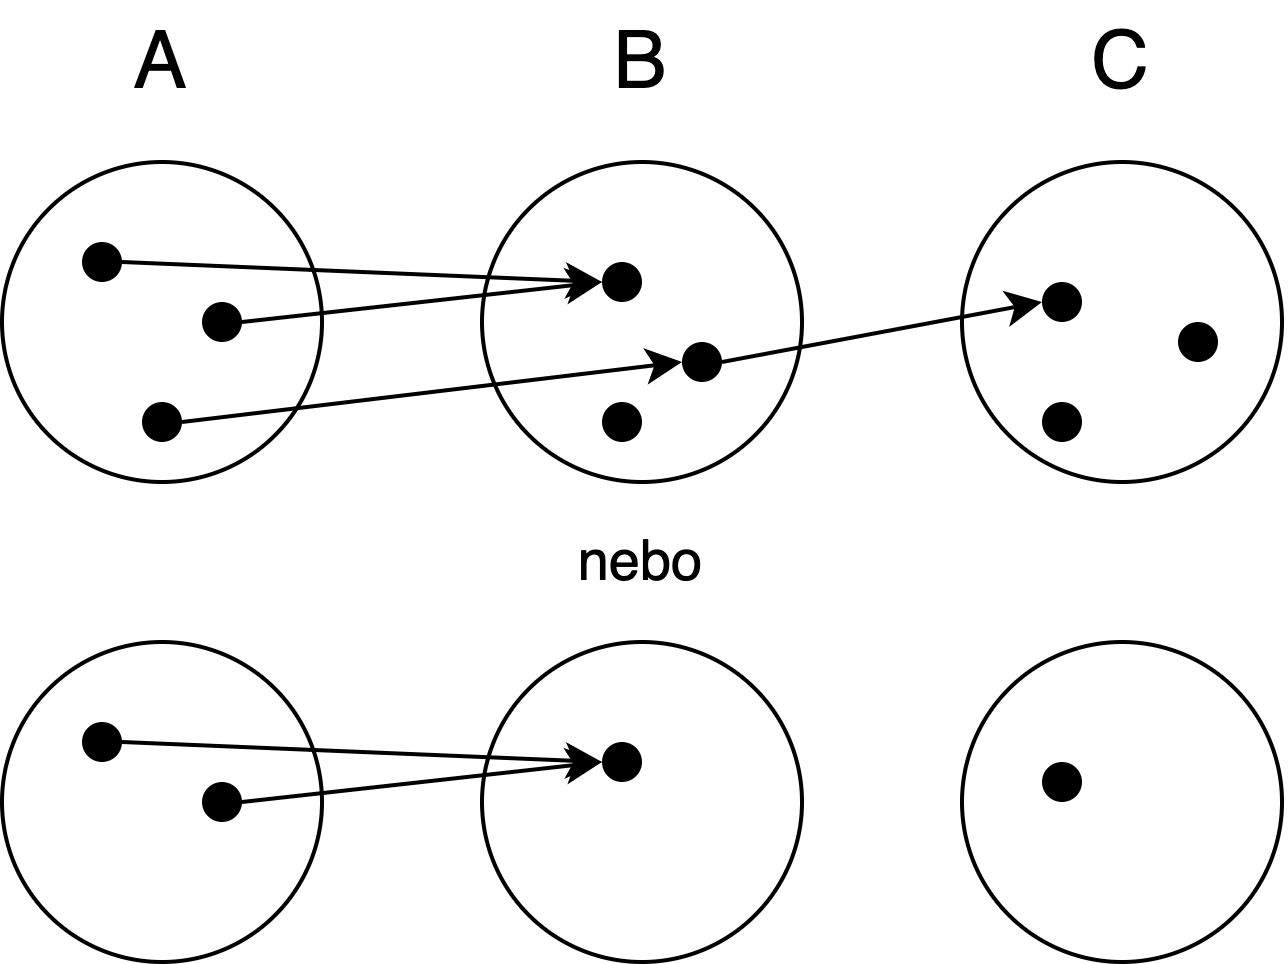
\includegraphics[scale=0.1]{figures/2022-0-2.drawio.png}
\end{center}

\question Např. \(\mathbb{F}_2\) s vektory \((0), (1)\).

\question Pokud je matice asymetrická, platí, že \(a_{i,j} = -a_{j,i}\). Pro diagonálu tedy musí platit, že je nulová, protože \(a = -a\). Stopa je tedy 0.

\question Pro \(V \in \mathbb{R}\), \(V \times V \rightarrow \mathbb{R}\) splňující \begin{itemize}
    \item Aditivitu
    \item Homogenitu
    \item Symetrii
    \item Pozitivní definitnost
\end{itemize}

\question Musí platit, že hodnost matice je stejná jako hodnot rozšířené matice.

}

\end{questions}
